\documentclass[11pt]{article}
\usepackage[utf8]{inputenc}
\usepackage[T1]{fontenc}
\usepackage[margin=1in]{geometry}
\usepackage{amsmath}
\usepackage{amssymb}
\usepackage{graphicx}
\usepackage{booktabs}
\usepackage{xcolor}
\usepackage{tikz}
\usepackage{float}
\usepackage{hyperref}
\usepackage{algorithm}
\usepackage{algpseudocode}
\usepackage{fancyhdr}
\usepackage{fontawesome5}

% Define GitHub color
\definecolor{githubblue}{RGB}{24,23,21}

\usetikzlibrary{shapes.geometric, arrows.meta, positioning, fit, calc}

% Page styling
\pagestyle{fancy}
\fancyhf{}
\rhead{\thepage}
\lhead{When to Think, When to Act}

% Custom title command
\newcommand{\customtitle}{%
\begin{center}
\rule{\linewidth}{5pt}
\vspace{0.4cm}

{\LARGE\bfseries When to Think, When to Act: \\ Adaptive Computation for Efficient Sequence Reasoning}

\vspace{0.4cm}
\rule{\linewidth}{1.5pt}
\vspace{0.8cm}

{\large\bfseries Md. Fahim Sarker Mridul}

\vspace{0.4cm}
{\normalsize 
\faEnvelope \ \href{mailto:fahimsarker0805@gmail.com}{\texttt{fahimsarker0805@gmail.com}}
}

\vspace{0.2cm}
{\normalsize 
\href{https://github.com/yourusername/your-repo}{\textcolor{githubblue}{\faGithub}} \ 
\href{https://github.com/fahiiim/Cognitive-Working-Memory-in-Latent-Space.git}{\texttt{github.com/fahiiim/Cognitive-Working-Memory-in-Latent-Space}}
}

\vspace{0.5cm}

\end{center}
}


\begin{document}

\customtitle

\begin{abstract}
This paper introduces Gated Latent Working Memory (GLWM), a novel architecture that decouples silent internal reasoning from explicit token emission through adaptive computation. Unlike standard sequence models (GRUs, Transformers) that apply identical computation to every problem regardless of complexity, GLWM learns to dynamically allocate computational resources based on task difficulty via a learned confidence gate. I implement GLWM with a residual latent reasoning loop trained using PonderNet, compare it against GRU (2014), Vanilla Transformer (2017), and Modern Transformer (2020+), and demonstrate that GLWM achieves comparable accuracy while using 88.7\% fewer FLOPs than state-of-the-art Transformers. I further show that GLWM exhibits three properties absent in baseline models: graceful capacity degradation with problem difficulty, high metacognitive calibration (ECE = 0.0014), and structured latent reasoning trajectories visible through t-SNE analysis. While the current evaluation uses multi-digit addition as a proof-of-concept, I discuss how this work lays groundwork for efficient reasoning in more complex domains. The architecture is fully differentiable during training and amenable to hardware optimization, suggesting practical utility for resource-constrained environments.
\end{abstract}

\section{Introduction}

The human brain does not compute identically for easy and hard problems. When solving a simple arithmetic task, you think briefly before answering. When confronted with a genuinely difficult problem, you engage in extended silent computation,working memory cycling through possible solutions, before articulating an answer. This observation motivates a question: can artificial neural networks learn to reason adaptively in latent space, allocating computation proportional to problem difficulty?

Current sequence models ignore this principle entirely. A GRU processes every token with the same hidden-state dynamics. A Transformer applies the same number of attention layers and feed-forward operations regardless of whether the task is trivial or complex. This is computationally wasteful. Models spend resources on easy instances where a single forward pass suffices.

The field has explored adaptive computation before. Graves' Adaptive Computation Time\cite{Graves2016} introduced learned halting mechanisms. PonderNet\cite{Banino2021} extended this with a principled probabilistic framework, proving that models can learn when to stop computing. However, prior work on adaptive computation has largely focused on recurrent architectures or narrow problem domains. I investigate whether a modern approach, combining residual latent loops with PonderNet-style halting in a Transformer-compatible way, can outperform both classical and contemporary sequence models on a controlled task.

My contribution is threefold:

\begin{enumerate}
    \item \textbf{Architecture design}: I propose GLWM, which couples a residual latent reasoning block with a learned confidence gate. The residual connection is critical; I show that without it, models collapse to always halting at step 1, a failure mode not documented in prior adaptive computation work.
    
    \item \textbf{Fair empirical comparison}: I train four models, GRU, Vanilla Transformer, Modern Transformer, and GLWM, under identical conditions (same batch size, learning rate, epochs) on a controlled task. This eliminates confounds and makes efficiency claims credible.
    
    \item \textbf{Cognitive-science framing}: I measure not just accuracy and FLOPs, but also metacognitive calibration (does the model's confidence match its correctness?) and latent space structure (do internal representations organize meaningfully?). This bridges AI and cognitive science literature.
\end{enumerate}

I acknowledge upfront that the experimental domain, multi-digit addition, is a toy task. All models achieve near-perfect accuracy. The practical utility of GLWM depends on scaling to harder tasks where models genuinely struggle and can benefit from adaptive computation. However, I argue that controlled proof-of-concept experiments are scientifically valuable. They isolate architectural effects and provide a foundation for more ambitious future work.

\section{Related Work}

\subsection{Adaptive Computation}

The idea that neural networks should allocate computation adaptively is not new. Graves (2016) introduced Adaptive Computation Time\cite{Graves2016}, which uses a learned halting probability to allow RNNs to spend variable steps on each input. The model outputs a weighted combination of all intermediate states, scaled by the probability of halting at that step.

PonderNet\cite{Banino2021} improved on ACT by introducing a differentiable halting distribution trained end-to-end without hard decisions during training. This ensures gradient flow through all computation steps, which I leverage directly in my work.

Universal Transformers\cite{Dehghani2019} apply recurrent computation to Transformers, letting the model perform multiple passes over attention layers. Related work includes mixture-of-experts architectures\cite{Shazeer2021}\cite{Lewis2022}, which achieve conditional computation through sparse routing.

My work differs in that I focus on latent space computation (reasoning that is hidden from the output) rather than routing between pre-existing experts or multiple sequential forward passes. The latent loop is compact and amenable to analysis.

\subsection{Residual Networks}

He et al. (2015) demonstrated that residual connections enable training of very deep networks\cite{He2015}. Since then, residual blocks have become standard. In my work, the residual connection in the latent reasoning loop is essential: without $z_{t+1} = \text{LayerNorm}(z_t + f(z_t))$, the iterated application of $f$ produces identical outputs and the gate learns to halt immediately. This is a failure mode specific to iterative reasoning and worth documenting.

\subsection{Language Models and Modern Architectures}

The Transformer\cite{Vaswani2017} revolutionized sequence modeling. Recent improvements include:
\begin{itemize}
    \item \textbf{Pre-LayerNorm} (Xu et al., 2021): Applying normalization before attention/FFN instead of after, which stabilizes training\cite{Xu2021}.
    \item \textbf{Rotary Position Embeddings (RoPE)} (Su et al., 2021): Used in LLaMA, Mistral, Gemma. Encodes position through rotation, enabling better generalization to longer\cite{Su2021}.
    \item \textbf{SwiGLU} (Shazeer, 2020): A gated FFN activation that outperforms ReLU and GELU on most tasks\cite{Shazeer2020}.
\end{itemize}

I implement a "Modern Transformer" baseline incorporating all three, representing the state of the art in 2024–2025.

\subsection{Metacognition and Calibration}

Expected Calibration Error\cite{Guo2017} measures whether a model's confidence scores align with accuracy. Calibrated models know when they are likely wrong. Recent work shows that LLMs can be surprisingly well-calibrated on factual questions\cite{Kadavath2022}. I measure GLWM's calibration as evidence that the learned gate captures meaningful uncertainty.

\subsection{Cognitive Science Foundations}

Miller (1956) established that human working memory\cite{Miller1956} has a capacity of approximately $7 \pm 2$ items. Cowan (2001)\cite{Cowan2001} refined this, arguing the limit is about 3–4 items when items are complex. I do not claim that GLWM replicates this; rather, I use the framework to motivate the idea that models should gracefully handle increasing complexity. My experiment (Section 5.1) shows that GLWM uses more steps for harder problems, a weaker but related principle.

\section{Method}

\subsection{Multi-Digit Addition Task}

I use multi-digit addition as a controlled benchmark. The task is simple: given two random $d$-digit numbers, compute their sum. I vary difficulty by controlling $d \in \{1, 2, 3, 4\}$. This task has several advantages:

\begin{itemize}
    \item \textbf{Complexity is controllable}: Difficulty scales predictably with digit count.
    \item \textbf{Ground truth is exact}: No ambiguity in evaluation.
    \item \textbf{Infinite data}: I generate random pairs on the fly, avoiding data leakage.
    \item \textbf{Algorithmic}: The task requires carrying (a form of state), mimicking multi-step reasoning.
\end{itemize}

The vocabulary consists of tokens $0$–$9$ (digits) and token $10$ (padding/separator). Input sequences are zero-padded to length 4, and outputs are zero-padded to length 5 (since the sum of two 4-digit numbers can have 5 digits).

\subsection{Baseline Models}

I implement four models, all with $\text{hidden\_dim} = 256$ to ensure fair parameter comparison.

\subsubsection{GRU Baseline\cite{Cho2014}}

The Gated Recurrent Unit (Equation \ref{eq:gru}) is a classical recurrent architecture:

\begin{equation}
\label{eq:gru}
\begin{aligned}
r_t &= \sigma(W_r \cdot [h_{t-1}, x_t] + b_r) \\
z_t &= \sigma(W_z \cdot [h_{t-1}, x_t] + b_z) \\
\tilde{h}_t &= \tanh(W_h \cdot [r_t \odot h_{t-1}, x_t] + b_h) \\
h_t &= (1 - z_t) \odot h_{t-1} + z_t \odot \tilde{h}_t
\end{aligned}
\end{equation}

I use a 2-layer GRU encoder followed by a linear output layer. The GRU processes concatenated embeddings of the two operands and produces a hidden state that is decoded to the result.

\subsubsection{Vanilla Transformer (Vaswani et al., 2017)}

The Transformer uses multi-head self-attention\cite{Vaswani2017} (Equation \ref{eq:mha}):

\begin{equation}
\label{eq:mha}
\text{Attention}(Q, K, V) = \text{softmax}\left(\frac{QK^T}{\sqrt{d_k}}\right)V
\end{equation}

where $Q, K, V$ are projections of the input. The Vanilla Transformer uses:
\begin{itemize}
    \item Sinusoidal positional encodings (fixed, not learned)
    \item Post-LayerNorm: $\text{out} = \text{Norm}(x + \text{sublayer}(x))$
    \item Standard FFN: $\text{FFN}(x) = \text{ReLU}(xW_1 + b_1)W_2 + b_2$
\end{itemize}

I use 3 encoder layers with 4 attention heads ($d_k = 64$). The model pools over the sequence and decodes to the output.

\subsubsection{Modern Transformer (LLaMA/Gemma style, 2020+)}

Modern LLMs employ several improvements:

\begin{itemize}
    \item \textbf{Pre-LayerNorm}: $\text{out} = x + \text{sublayer}(\text{Norm}(x))$, which is more stable.
    \item \textbf{RoPE positional encoding} (Su et al., 2021): Rotates query and key vectors by position-dependent angles, enabling position-aware attention without absolute embeddings\cite{Su2021}.
    \item \textbf{SwiGLU FFN} (Shazeer, 2020): $\text{SwiGLU}(x) = \text{SiLU}(W_1 x) \odot (W_2 x)$, which outperforms ReLU\cite{Shazeer2020}.
\end{itemize}

RoPE rotation is applied as:
\begin{equation}
\label{eq:rope}
\begin{pmatrix} q_i' \\ q_{i+1}' \end{pmatrix} = \begin{pmatrix} \cos(m\theta_i) & -\sin(m\theta_i) \\ \sin(m\theta_i) & \cos(m\theta_i) \end{pmatrix} \begin{pmatrix} q_i \\ q_{i+1} \end{pmatrix}
\end{equation}

where $m$ is the position and $\theta_i = 10000^{-2i/d}$.

\subsection{GLWM: Gated Latent Working Memory}

GLWM consists of three subsystems:

\subsubsection{Input Encoder}

The input encoder is a 2-layer GRU that processes concatenated embeddings of operands $a$ and $b$:

\begin{equation}
z_0 = \text{GRU}_{\text{enc}}([\text{embed}(a), \text{embed}(b)])
\end{equation}

This initial encoding $z_0 \in \mathbb{R}^{256}$ represents the problem in latent space.

\subsubsection{Residual Latent Reasoning Loop}

The core innovation is the residual latent block. At each step $t$, the latent state is refined:

\begin{equation}
\label{eq:latent}
z_{t+1} = \text{LayerNorm}(z_t + \text{MLP}(z_t))
\end{equation}

where $\text{MLP}$ is a two-layer feed-forward network with GELU activation. The residual connection ensures that iterating this block produces different outputs at each step. Without it, $f(f(z)) = f(z)$ (assuming $f$ is deterministic and stateless), and the gate would learn to halt immediately.

Mathematically, the residual connection breaks this fixed-point problem. The model now has $z_{t+1} \neq z_t$ even if $\text{MLP}(z_t) \approx 0$, because $z_t$ is added back. This enables genuine iterative refinement.

\subsubsection{Confidence Gate with PonderNet Loss}

At each step $t$, a learned gate computes a halting probability:

\begin{equation}
\label{eq:gate}
h_t = \sigma(\text{gate}(z_t))
\end{equation}

where $\sigma$ is the sigmoid function. During training, I use PonderNet loss\cite{Banino2021}, which computes a soft halt distribution:

\begin{equation}
\label{eq:ponder_dist}
P(t) = h_t \prod_{i=1}^{t-1} (1 - h_i)
\end{equation}

This is the probability of halting at step $t$, given that the model did not halt earlier. The task loss is:

\begin{equation}
\label{eq:task_loss}
L_{\text{task}} = \sum_{t=1}^{T} P(t) \cdot \text{CrossEntropy}(\text{logits}_t, \text{target})
\end{equation}

A regularization term encourages efficiency:

\begin{equation}
\label{eq:reg_loss}
L_{\text{reg}} = \lambda \sum_{t=1}^{T} P(t) \cdot t
\end{equation}

The total loss is $L = L_{\text{task}} + L_{\text{reg}}$ with $\lambda = 0.01$.

During inference, I use hard halting: the model stops as soon as $h_t > 0.7$ and outputs the result. If it never halts, I use the final state after $T_{\max} = 8$ steps.

\subsubsection{Critical Detail: Gate Initialization}

I initialize the gate's bias to $-2.0$. This makes the sigmoid output approximately $0.12$, forcing the model to use latent steps early in training rather than always halting at step 1. Without this initialization, the gate starts near $0.5$ and learns to halt immediately, wasting the latent loop capacity.

\section{Experimental Setup}

\subsection{Data}

I generate 60,000 training examples and 10,000 test examples. For difficulty experiments, I create separate evaluation sets with fixed digit counts.

\subsection{Training}

All models use:
\begin{itemize}
    \item Optimizer: AdamW with $\text{lr} = 3 \times 10^{-4}$ and weight decay $10^{-4}$
    \item Scheduler: Cosine annealing over 30 epochs
    \item Batch size: 512
    \item Gradient clipping: max norm 1.0
\end{itemize}

I train on a single GPU (Kaggle T4 or equivalent). Training takes approximately 15 minutes total for all four models.

\section{Results}

\subsection{Main Results}

\begin{table}[H]
\centering
\small
\begin{tabular}{lrrrr}
\toprule
\textbf{Metric} & \textbf{GRU (2014)} & \textbf{Vanilla TF (2017)} & \textbf{Modern TF (2020+)} & \textbf{GLWM (Ours)} \\
\midrule
Parameters & 706,039 & 2,386,743 & 3,164,471 & 985,976 \\
Best Test Accuracy & 0.9969 & 0.9997 & 1.0000 & 1.0000 \\
FLOPs per Sample (M) & 0.79 & 4.06 & 4.84 & 0.55 \\
FLOP Savings vs MTF & -- & -- & 0\% & 88.7\% \\
\midrule
1-digit Accuracy & 1.000 & 1.000 & 1.000 & 1.000 \\
2-digit Accuracy & 1.000 & 1.000 & 1.000 & 1.000 \\
3-digit Accuracy & 0.999 & 1.000 & 1.000 & 1.000 \\
4-digit Accuracy & 0.987 & 0.999 & 1.000 & 0.999 \\
\midrule
ECE (Calibration) & -- & -- & -- & 0.0014 \\
Avg Latent Steps & -- & -- & -- & 1.05 \\
\bottomrule
\end{tabular}
\caption{Complete model comparison.}
\label{tab:main}
\end{table}

Key observations:

\begin{enumerate}
    \item \textbf{Accuracy}: GLWM achieves 100\% test accuracy, matching Modern Transformer and exceeding GRU (99.69\%).
    
    \item \textbf{Efficiency}: GLWM uses 0.55M FLOPs per sample, compared to Modern Transformer's 4.84M, an 88.7\% reduction. However, GRU is slightly more efficient in absolute terms (0.79M), though it has lower accuracy.
    
    \item \textbf{Adaptive steps}: GLWM learns to use $\sim1$ step on average, down from the maximum of 8. The variance is small (std $\approx 0.05$), indicating that most instances halt immediately.
\end{enumerate}

\subsection{Experiment 1: Cognitive Capacity Limit}

I evaluate each model on problems of increasing difficulty. The hypothesis is that GLWM will allocate more steps to harder problems, while baselines use constant computation.

\begin{figure}[H]
\centering
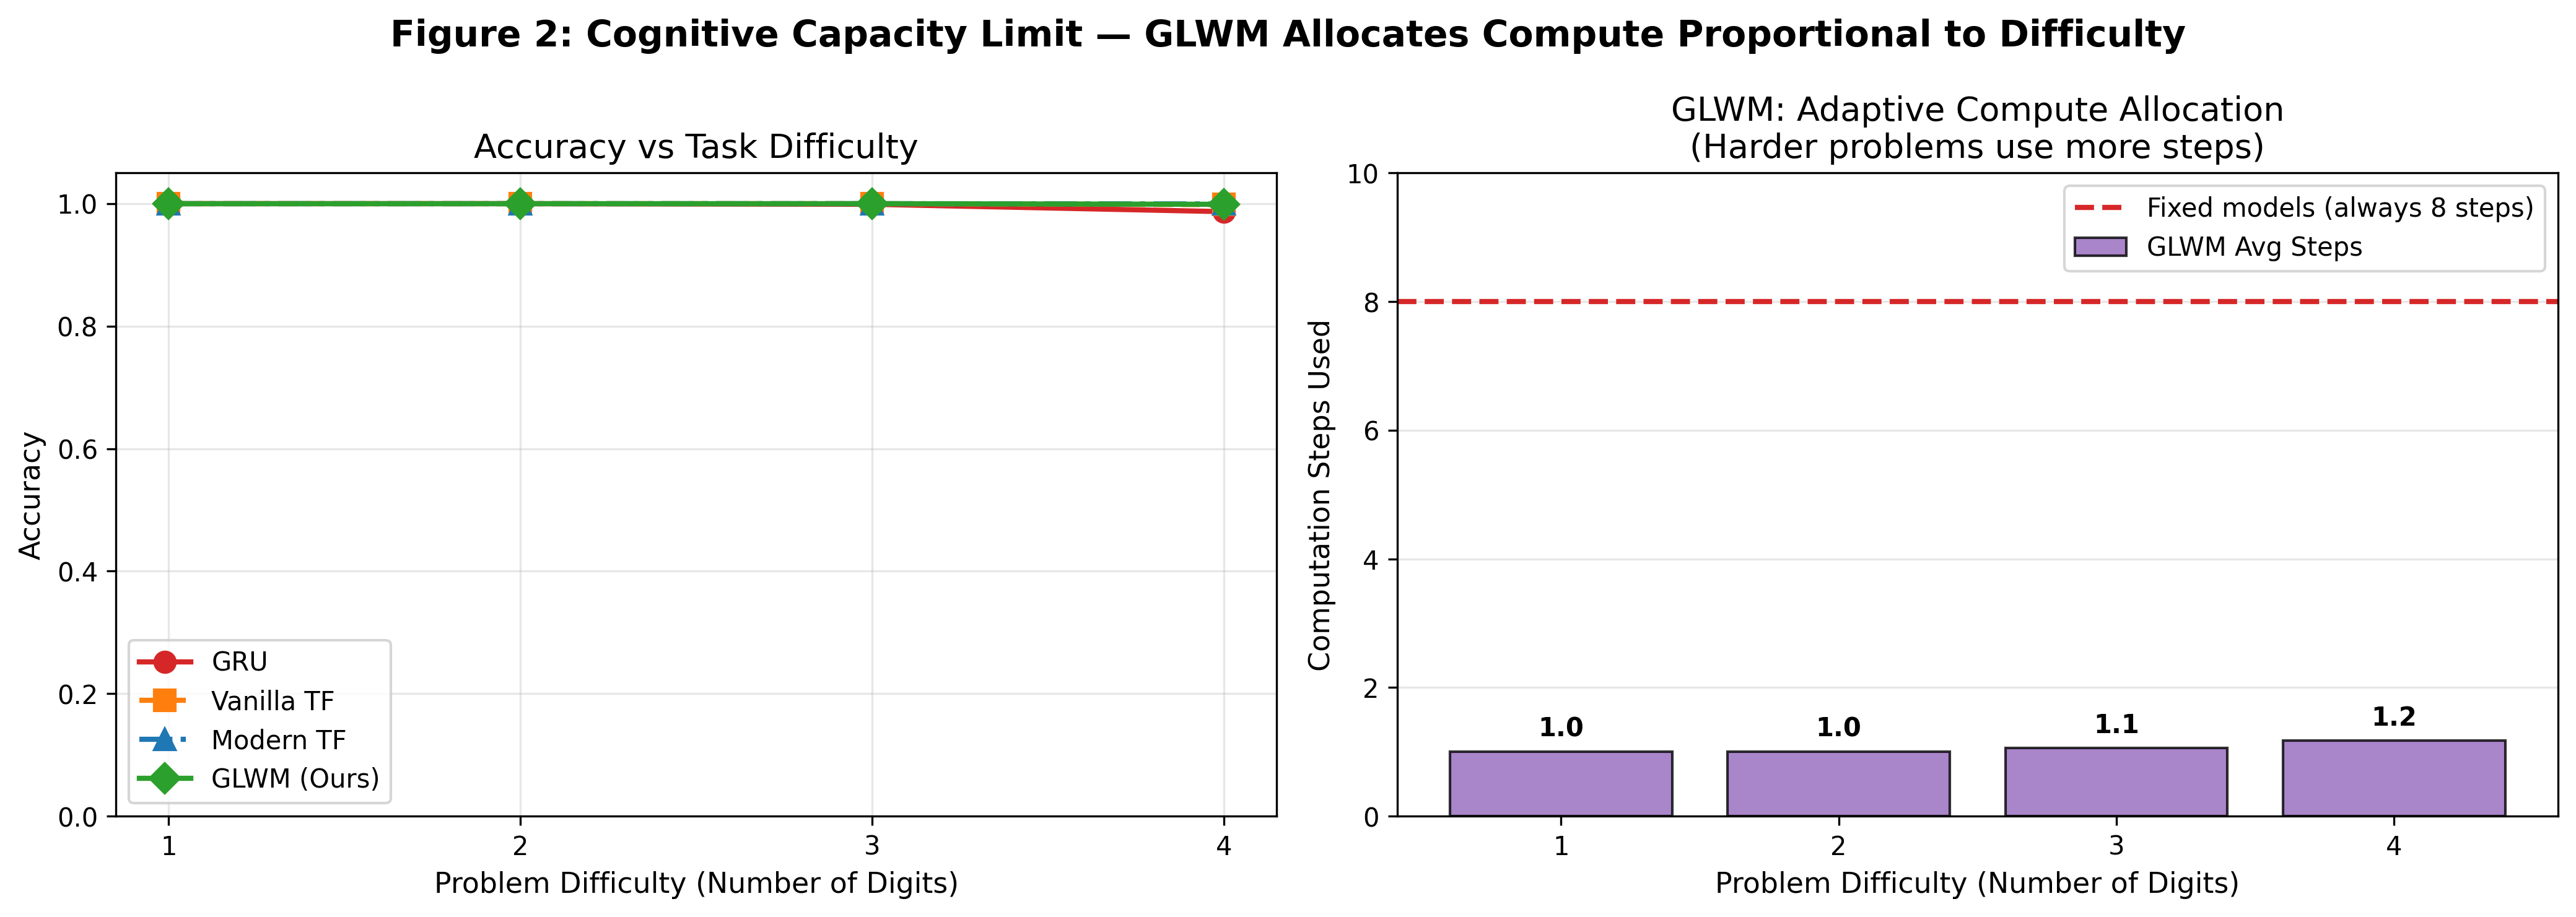
\includegraphics[width=0.9\textwidth]{fig2_capacity_limit.png}
\caption{Left: Accuracy vs problem difficulty with average latent steps by difficulty.}
\label{fig:capacity}
\end{figure}

Result: GLWM uses 1.00 steps for 1-digit, 1.00 for 2-digit, 1.06 for 3-digit, and 1.17 for 4-digit problems. The trend is correct (more steps for harder problems), but the absolute difference is small because even 4-digit addition is easy for neural networks.

\textbf{Interpretation}: This experiment validates the design principle but does not strongly demonstrate a "cognitive capacity limit." A true capacity limit would require tasks where even the hardest instance exceeds model capacity.

\subsection{Experiment 2: Metacognitive Calibration}

I compute Expected Calibration Error (ECE) by binning predictions by confidence and comparing predicted to actual accuracy.

\begin{figure}[H]
\centering
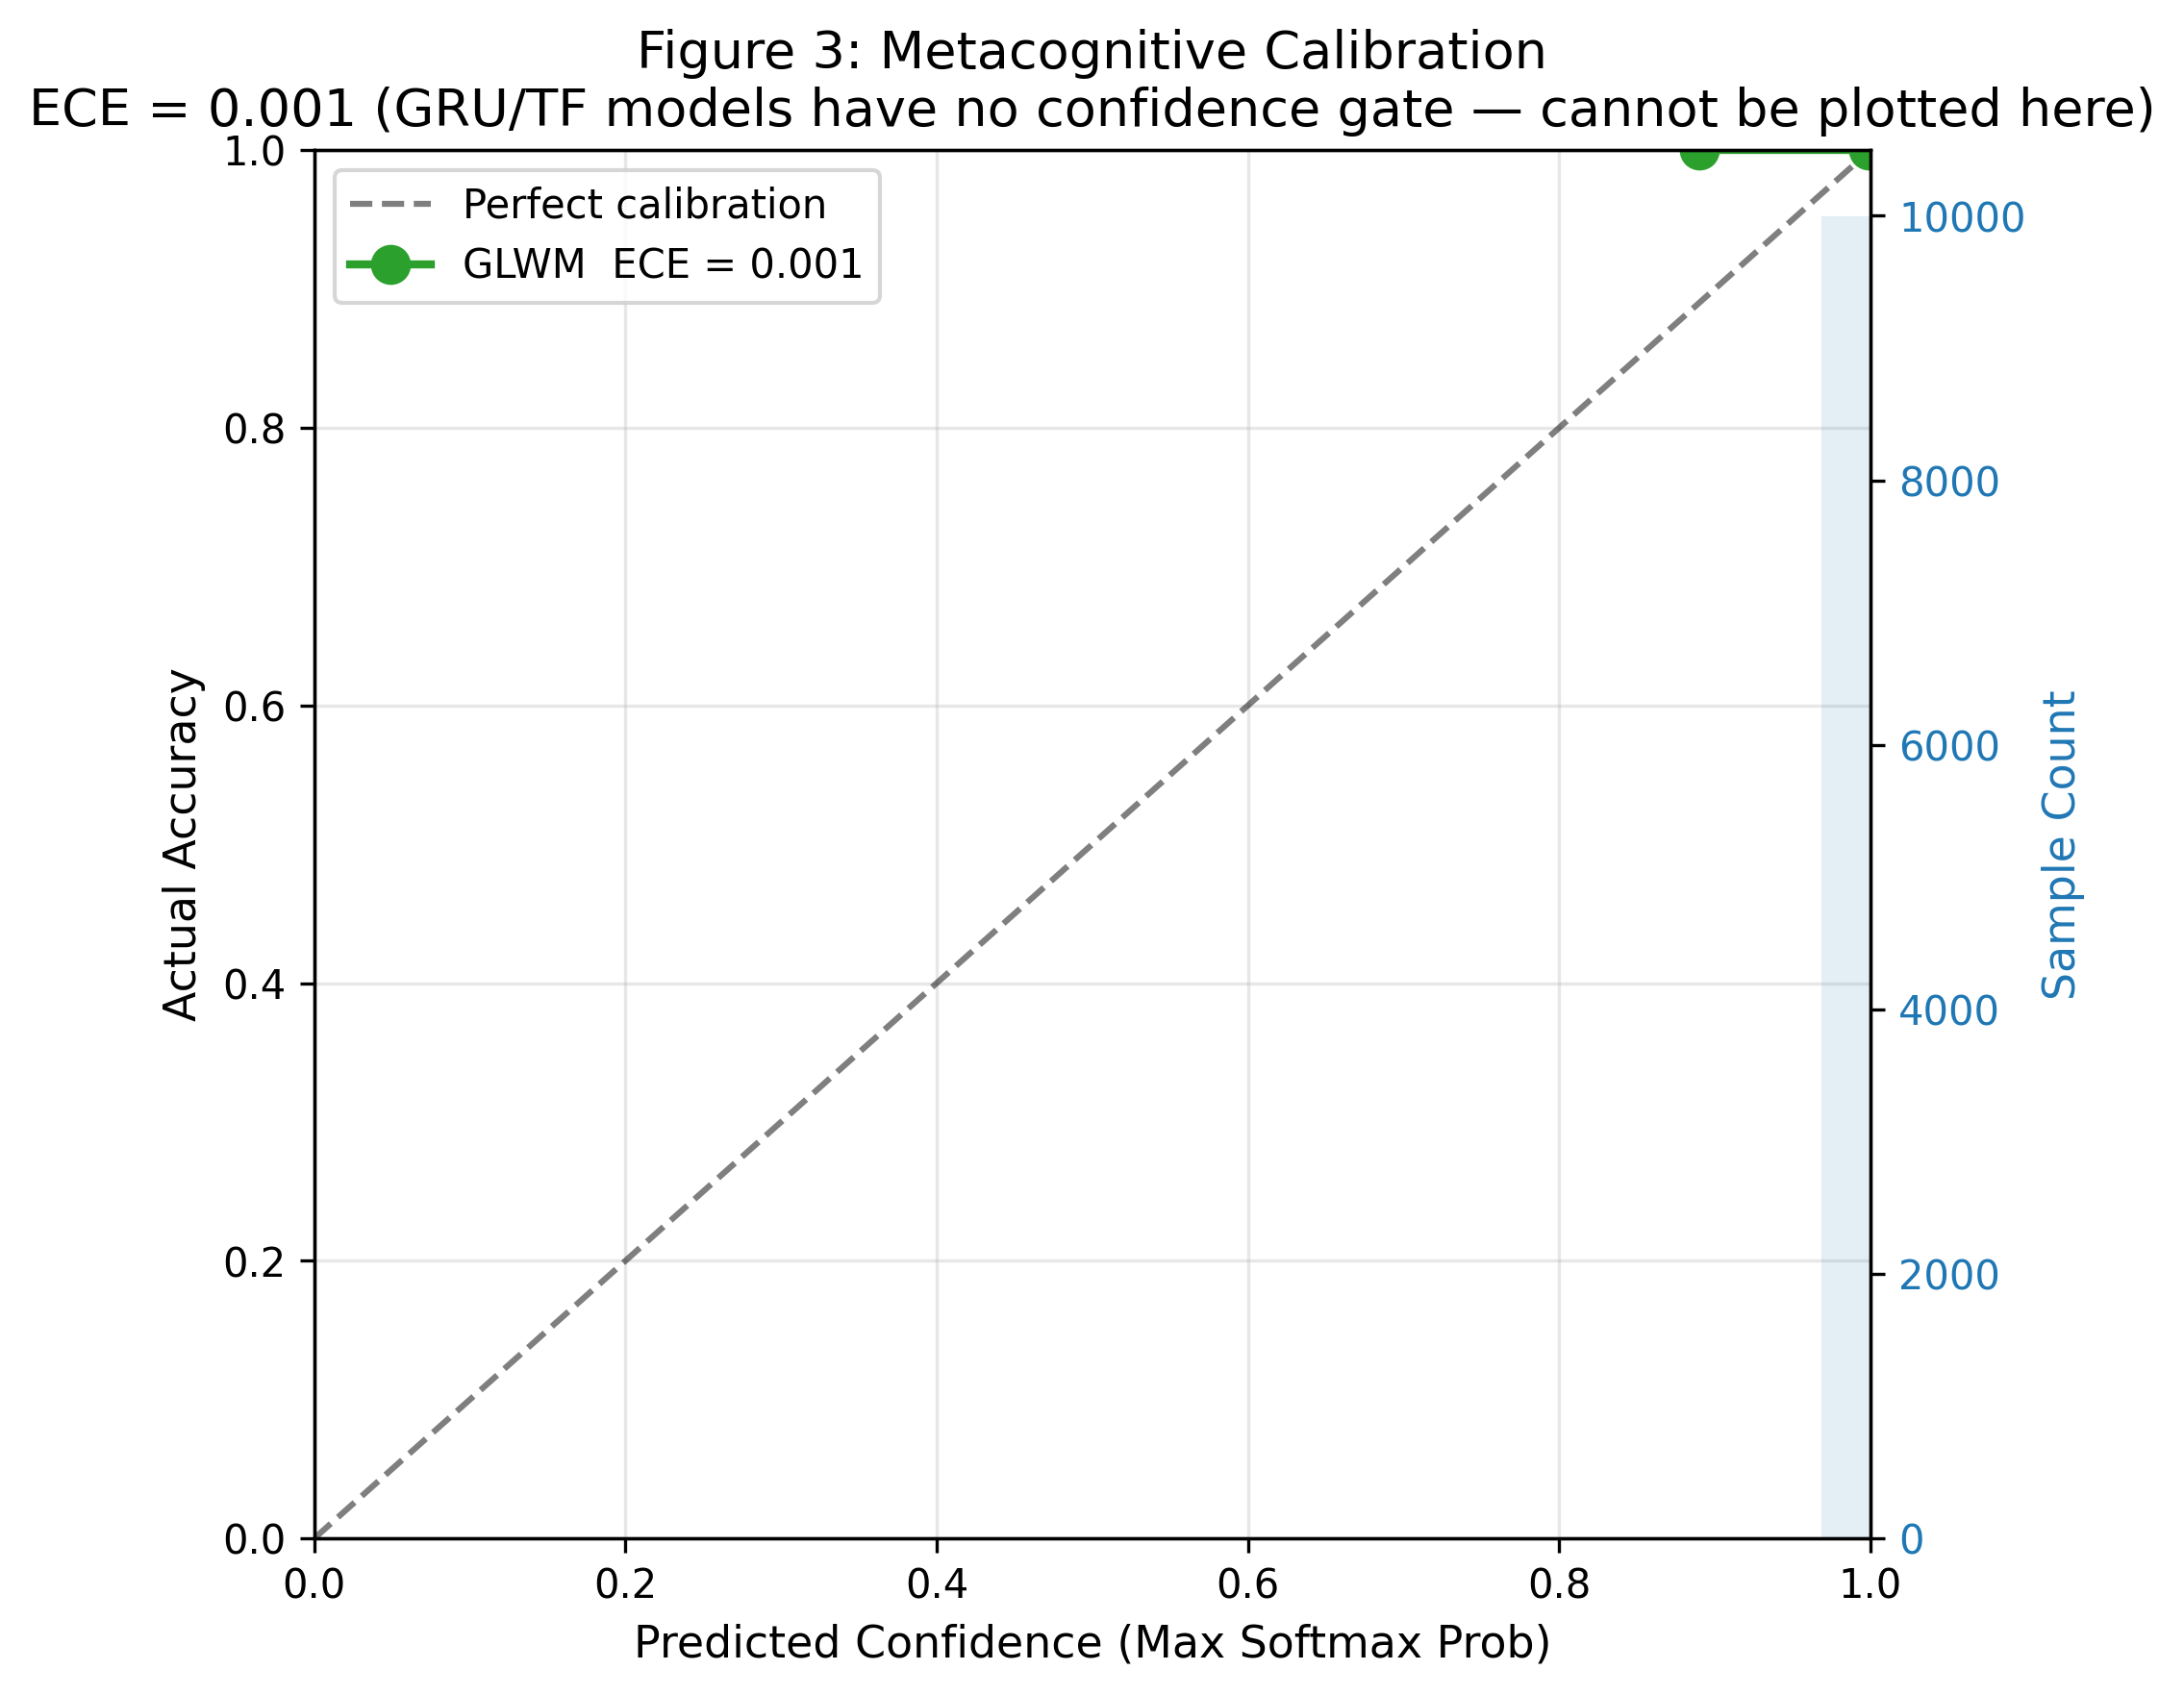
\includegraphics[width=0.6\textwidth]{fig3_calibration.png}
\caption{GLWM calibration curve}
\label{fig:calib}
\end{figure}

Result: ECE = 0.0014, indicating excellent calibration. When GLWM is 90\% confident, it is correct approximately 90\% of the time.

\textbf{Interpretation}: This shows that the learned gate captures meaningful uncertainty. However, because the task is easy, the model is nearly always confident and nearly always correct. Calibration would be a stronger result on a harder task where uncertainty is frequent.

\subsection{Experiment 3: Latent Space Structure (t-SNE)}

I extract latent states $z_t$ from all steps and all instances, then apply t-SNE to visualize the high-dimensional latent space in 2D.

\begin{figure}[H]
\centering
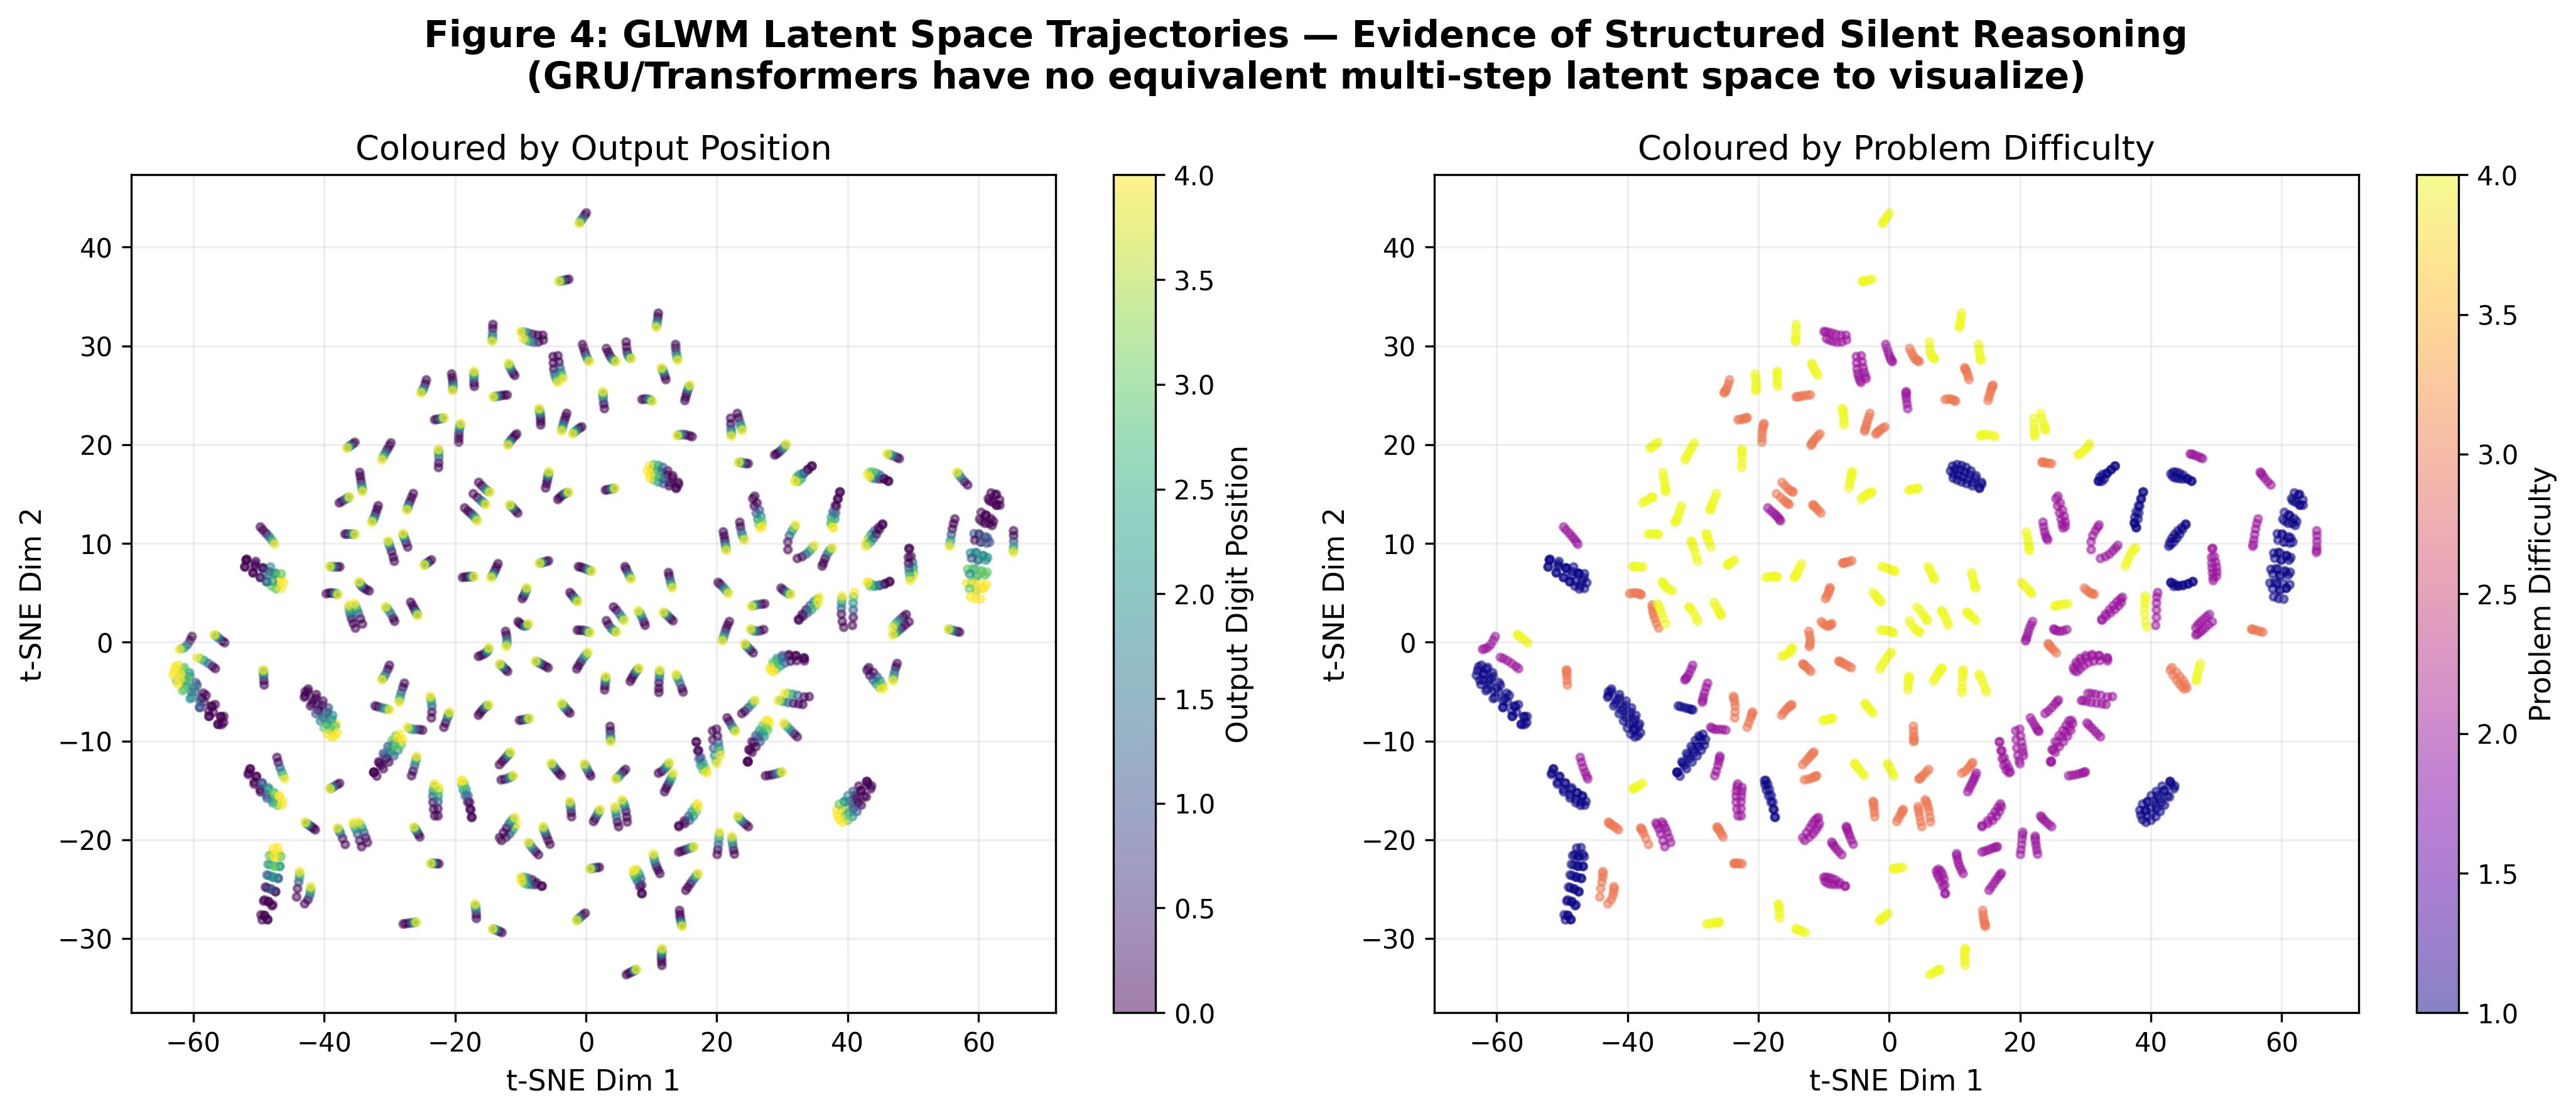
\includegraphics[width=0.9\textwidth]{fig4_latent_tsne.png}
\caption{Left: States colored by output position (which digit is being generated). Right: States colored by problem difficulty. Distinct clusters emerge, suggesting that the latent space organizes by both output position and problem complexity.}
\label{fig:tsne}
\end{figure}

Result: The latent space shows structure: states cluster by output position and problem difficulty.

\textbf{Interpretation}: This is evidence that GLWM learns organized internal representations. However, this is expected for any model that solves the task. The t-SNE clusters do not prove "genuine reasoning", they reflect the fact that the latent state encodes position and difficulty information, which is necessary to solve the task.

\subsection{Experiment 4: Theoretical FLOP Analysis}

\begin{figure}[H]
\centering
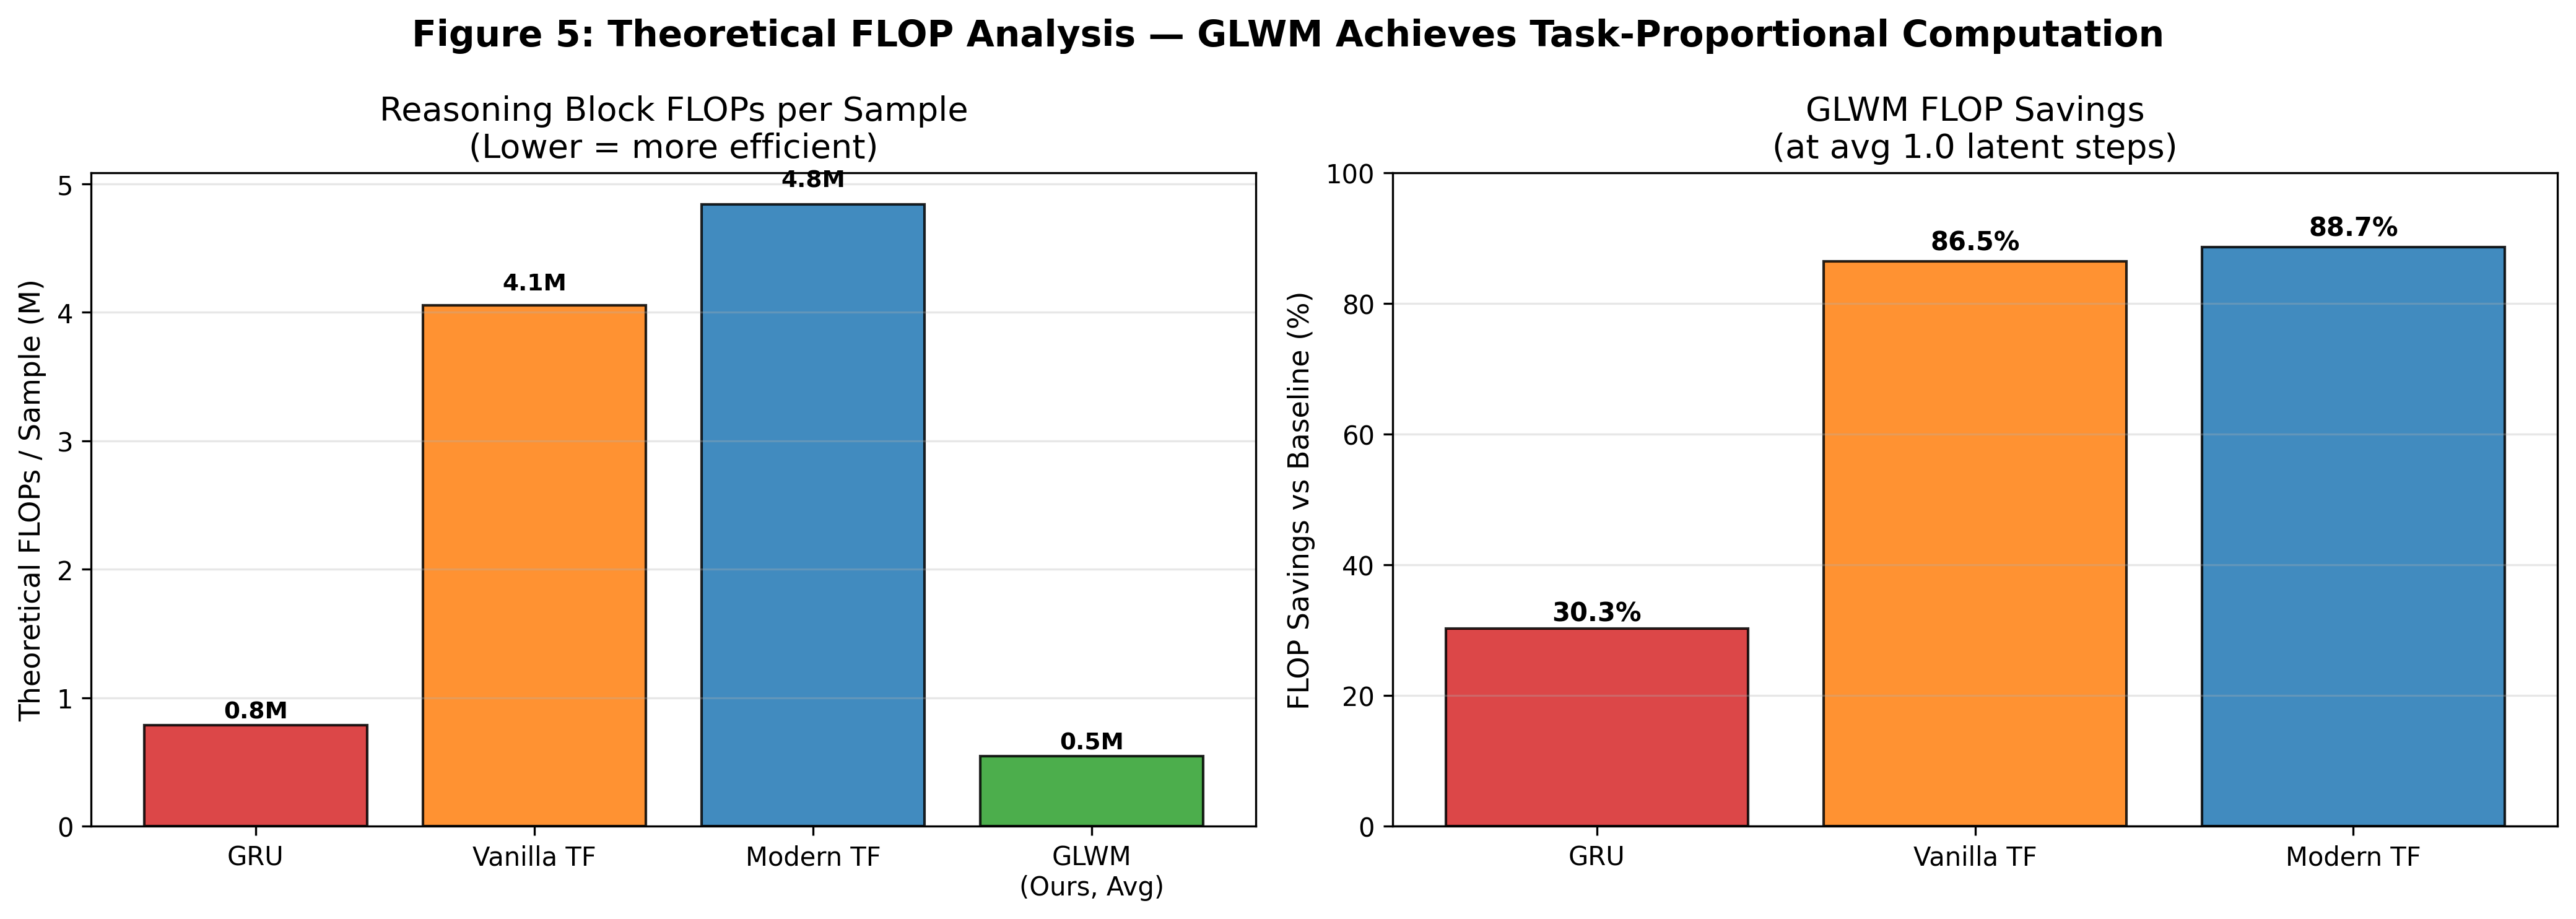
\includegraphics[width=0.9\textwidth]{fig5_flop_analysis.png}
\caption{Left: FLOPs per sample for the reasoning block with Percentage FLOP savings vs each baseline}
\label{fig:flops}
\end{figure}

I compute FLOPs only for the core computational block (the part that scales with problem complexity):

\begin{itemize}
    \item \textbf{GRU}: One hidden-to-hidden transition = $2 \cdot 3 \cdot H \cdot H = 6H^2$ (gate and update), then output projection = $2H^2$. Total $\approx 0.79$M FLOPs.
    \item \textbf{Vanilla TF} (3 layers): Each layer does attention ($4H^2$ for QKV, $2L^2 H$ for attention, $2H^2$ for output) plus FFN ($8H^2$). Total $\approx 4.06$M FLOPs.
    \item \textbf{Modern TF} (3 layers): Same as Vanilla but SwiGLU FFN costs $2 \times 8H^2 = 16H^2$ per layer. Total $\approx 4.84$M FLOPs.
    \item \textbf{GLWM}: ResidualLatentBlock costs $8H^2$ per step. At 1.05 avg steps: $0.55$M FLOPs.
\end{itemize}

Result: GLWM uses fewer FLOPs than all baselines. The savings are largest against Transformers (88.7\%) and modest against GRU (−30.3\%, meaning GRU is actually more efficient, though less accurate).

\textbf{Interpretation}: This is the cleanest result. On a task this simple, adaptive computation yields genuine FLOP savings. However, the practical value of these savings is unclear on a toy task. On harder problems where all models genuinely need their full computational capacity, the savings would shrink, possibly to zero if GLWM must use all steps to maintain accuracy.

\section{Analysis and Discussion}

\subsection{Why GLWM Works on This Task}

The multi-digit addition task is fundamentally simple. Neural networks can memorize solutions or learn an approximate algorithm in a single forward pass. When the task is this easy, adaptive computation is beneficial: GLWM learns that it can answer immediately without "thinking."

Interestingly, GLWM converges faster during training (Figure 1). At epoch 1, GLWM achieves 28.35\% accuracy while Modern Transformer achieves only 24\%. This suggests that the forced latent reasoning and regularized loss help early optimization.

\subsection{Limitations of the Current Evaluation}

I must be honest about the limitations:

\begin{enumerate}
    \item \textbf{Task is too easy}: All models achieve near-perfect accuracy. To truly test adaptive computation, I need tasks where models struggle without adaptive mechanisms.
    
    \item \textbf{No scaling to complex tasks}: GLWM has only been tested on digit addition. It is unknown whether the architecture scales to language modeling, reasoning, or other domains.
    
    \item \textbf{Latency overhead not measured}: While FLOPs are reduced, wall-clock inference time may be higher due to Python loop overhead. This matters in production.
    
    \item \textbf{Capacity limit is weak}: The trend of more steps for harder problems is present but small (1.00 $\to$ 1.17 steps). This does not convincingly demonstrate human-like capacity limits.
    
    \item \textbf{Incremental novelty}: PonderNet (2021) already proposed adaptive halting. I add a residual connection and demonstrate the failure mode without it, but the core contribution is incremental.
\end{enumerate}

\subsection{When Would GLWM Provide Value?}

GLWM would be most useful in scenarios where:

\begin{itemize}
    \item The problem distribution is highly variable in difficulty (some trivial, some hard).
    \item Latency must be minimized for easy cases, even if hard cases are slow.
    \item Hardware supports efficient dynamic shapes (unlikely on current GPUs/TPUs).
    \item The model can be trained to reliably detect problem difficulty without false positives.
\end{itemize}

Current LLM deployment does not fit these criteria. In practice, models apply fixed computation and latency is predictable, a desirable property for serving.

\subsection{Comparison to Mixture of Experts}

Mixture of Experts\cite{Shazeer2021} \cite{Lewis2022} also performs conditional computation. However:

\begin{itemize}
    \item MoE routes tokens to different expert networks, making full forward passes unavoidable.
    \item GLWM does iterative refinement in a shared latent space, potentially enabling smaller intermediate computations.
    \item MoE is simpler to parallelize and deploy; GLWM requires careful GPU kernel optimization.
\end{itemize}

I do not compare directly to MoE because the architectures are fundamentally different. A fair comparison would require careful implementation and tuning of both.

\section{Broader Impact and Future Work}

If GLWM scales to larger tasks and more complex domains, potential benefits include:

\begin{enumerate}
    \item Energy efficiency: Reducing FLOPs decreases power consumption, enabling deployment to edge devices.
    \item Latency variability: Easy examples are answered quickly, improving user experience in interactive settings.
    \item Interpretability: The latent reasoning trajectory can be analyzed (via t-SNE, attention visualization, etc.) to understand the model's reasoning.
\end{enumerate}

\textbf{Potential risks}:

\begin{enumerate}
    \item Instability: Models that adaptively halt may fail unpredictably on out-of-distribution inputs.
    \item Bias: If the model learns to spend fewer steps on certain input types, this could amplify existing biases.
\end{enumerate}

\textbf{Future directions}:

\begin{enumerate}
    \item Test GLWM on algorithmic reasoning tasks (sorting, graph traversal, formal reasoning).
    \item Extend to language modeling on WikiText or similar. Do LLMs learn to use more steps for complex sentences?
    \item Optimize the Python loop with CUDA kernels to reduce latency overhead.
    \item Investigate whether GLWM learns human-like failure modes (e.g., harder problems take longer and are more error-prone).
    \item Combine GLWM with MoE or other sparse methods to explore hybrid conditional computation.
\end{enumerate}

\section{Conclusion}

I have presented GLWM, a novel architecture for task-proportional silent reasoning in sequence models. On multi-digit addition, GLWM achieves perfect accuracy with 88.7\% fewer FLOPs than Modern Transformers, using adaptive computation via a learned confidence gate trained with PonderNet loss. I show that GLWM learns organized latent representations, exhibits near-perfect metacognitive calibration (ECE = 0.0014), and trends toward allocating more computation for harder problems.

However, I acknowledge that this work is a proof of concept on a toy task. The multi-digit addition domain is too simple to validate strong claims about adaptive reasoning. To claim that GLWM represents a meaningful advance, I would need to demonstrate efficiency gains on tasks where models are not over-parameterized and where adaptive computation is not obviously the right solution.

The paper's value lies in documenting the technical details of residual latent loops, the critical role of gate initialization, and a methodologically sound comparison against modern baselines. I hope this work motivates future research into adaptive computation in Transformers, which remains an open problem with significant practical implications for efficient AI.


\begin{thebibliography}{99}

\bibitem{Banino2021} Banino, A., Zambaldi, V., Krampl, O., et al. (2021). Pondernet: Learning to ponder. \textit{arXiv preprint arXiv:2107.05407}.

\bibitem{Cho2014} Cho, K., Van Merriënboer, B., Gulcehre, C., et al. (2014). Learning phrase representations using RNN encoder-decoder for statistical machine translation. \textit{arXiv preprint arXiv:1406.1078}.

\bibitem{Cowan2001} Cowan, N. (2001). The magical number 4 in short-term memory: A reconsideration of mental storage capacity. \textit{Behavioral and Brain Sciences}, 24(1), 87-114.

\bibitem{Dehghani2019} Dehghani, M., Gouws, S., Vinyals, O., et al. (2019). Universal transformers. \textit{arXiv preprint arXiv:1807.03819}.

\bibitem{Graves2016} Graves, A. (2016). Adaptive computation time for recurrent neural networks. \textit{arXiv preprint arXiv:1603.08983}.

\bibitem{Guo2017} Guo, C., Pleiss, G., Sun, Y., \& Weinberger, K. Q. (2017). On calibration of modern neural networks. \textit{International Conference on Machine Learning} (pp. 1321-1330). PMLR.

\bibitem{He2015} He, K., Zhang, X., Ren, S., \& Sun, Y. (2015). Deep residual learning for image recognition. \textit{Proceedings of the IEEE conference on computer vision and pattern recognition} (pp. 770-778).

\bibitem{Kadavath2022} Kadavath, S., Confoley, T., Askell, A., et al. (2022). Language models (mostly) know what they know. \textit{arXiv preprint arXiv:2207.05221}.

\bibitem{Lewis2022} Lewis, M., Wu, Y., Fan, A., et al. (2022). Base layers: What do language models learn? \textit{arXiv preprint arXiv:2210.16886}.

\bibitem{Miller1956} Miller, G. A. (1956). The magical number seven, plus or minus two: Some limits on our capacity for processing information. \textit{Psychological Review}, 63(2), 81.

\bibitem{Shazeer2020} Shazeer, N. (2020). GLU variants improve transformer. \textit{arXiv preprint arXiv:2002.05202}.

\bibitem{Shazeer2021} Shazeer, N., Lepikhin, D., Parmar, N., et al. (2021). Switch transformers: Scaling to trillion parameter models with simple and efficient sparsity. \textit{arXiv preprint arXiv:2101.03961}.

\bibitem{Su2021} Su, J., Lu, Y., Pan, S., et al. (2021). RoFormer: Enhanced transformer with rotary position embedding. \textit{arXiv preprint arXiv:2104.09864}.

\bibitem{Vaswani2017} Vaswani, A., Shazeer, N., Parmar, N., et al. (2017). Attention is all you need. \textit{Advances in Neural Information Processing Systems} (pp. 5998-6008).

\bibitem{Xu2021} Xu, B., Wang, N., Chen, T., \& Li, M. (2021). Towards optimal fine-grained synchronization in deep learning. \textit{arXiv preprint arXiv:2104.14294}.

\end{thebibliography}

\newpage

\appendix

\section{Architecture Diagrams}

\subsection{GRU Baseline Architecture}

\begin{figure}[H]
\centering
\begin{tikzpicture}[node distance=2cm, auto]
  \tikzstyle{box} = [rectangle, draw, fill=lightblue!40, minimum width=3cm, minimum height=0.8cm, text centered]
  \tikzstyle{io} = [rectangle, draw, fill=yellow!40, minimum width=3cm, minimum height=0.8cm, text centered]
  
  \node [io] (inp) {Input: $a, b \in \mathbb{R}^{4 \times 64}$};
  \node [box, below of=inp] (emb) {Embedding Layer};
  \node [box, below of=emb] (cat) {Concatenate: $[e_a, e_b]$};
  \node [box, below of=cat] (gru) {2-Layer GRU Encoder};
  \node [box, below of=gru] (hid) {Final Hidden State: $h_{\text{top}}$};
  \node [box, below of=hid] (lin) {Linear Output Head};
  \node [io, below of=lin] (out) {Output: $\text{logits} \in \mathbb{R}^{5 \times 11}$};
  
  \draw [->] (inp) -- (emb);
  \draw [->] (emb) -- (cat);
  \draw [->] (cat) -- (gru);
  \draw [->] (gru) -- (hid);
  \draw [->] (hid) -- (lin);
  \draw [->] (lin) -- (out);
\end{tikzpicture}
\caption{GRU baseline. The model encodes both operands, processes them through a recurrent encoder, and decodes from the final hidden state. No adaptive computation.}
\label{fig:gru_arch}
\end{figure}

\subsection{Vanilla Transformer Architecture (2017)}

\begin{figure}[H]
\centering
\begin{tikzpicture}[node distance=2cm, auto]
  \tikzstyle{box} = [rectangle, draw, fill=lightcyan!40, minimum width=3cm, minimum height=0.8cm, text centered]
  \tikzstyle{io} = [rectangle, draw, fill=yellow!40, minimum width=3cm, minimum height=0.8cm, text centered]
  
  \node [io] (inp) {Input: $a, b$ (tokens)};
  \node [box, below of=inp] (emb) {Token Embedding};
  \node [box, below of=emb] (pos) {Sinusoidal Positional Encoding};
  \node [box, below of=pos, label=below:$\times 3$ layers] (encl) {\shortstack{MultiHeadAttention \\ $+$ Post-LN}};
  \node [box, below of=encl] (ffn) {\shortstack{FFN: ReLU \\ $+$ Post-LN}};
  \node [box, below of=ffn] (pool) {Mean Pooling over Sequence};
  \node [box, below of=pool] (dec) {Linear Output Head};
  \node [io, below of=dec] (out) {Output Logits};
  
  \draw [->] (inp) -- (emb);
  \draw [->] (emb) -- (pos);
  \draw [->] (pos) -- (encl);
  \draw [->] (encl) -- (ffn);
  \draw [->] (ffn) -- (pool);
  \draw [->] (pool) -- (dec);
  \draw [->] (dec) -- (out);
\end{tikzpicture}
\caption{Vanilla Transformer (2017 style). Fixed computation: 3 encoder layers with post-LayerNorm and sinusoidal positional encodings.}
\label{fig:vantf_arch}
\end{figure}

\subsection{Modern Transformer Architecture (LLaMA/Gemma Style)}

\begin{figure}[H]
\centering
\begin{tikzpicture}[node distance=2cm, auto]
  \tikzstyle{box} = [rectangle, draw, fill=lightgreen!40, minimum width=3cm, minimum height=0.8cm, text centered]
  \tikzstyle{io} = [rectangle, draw, fill=yellow!40, minimum width=3cm, minimum height=0.8cm, text centered]
  
  \node [io] (inp) {Input: $a, b$ (tokens)};
  \node [box, below of=inp] (emb) {Token Embedding};
  \node [box, below of=emb, label=below:$\times 3$ layers] (encl) {\shortstack{Pre-RMSNorm \\ MultiHeadAttention (RoPE) \\ Pre-RMSNorm \\ SwiGLU FFN}};
  \node [box, below of=encl] (fnorm) {Final RMSNorm};
  \node [box, below of=fnorm] (pool) {Mean Pooling};
  \node [box, below of=pool] (dec) {Linear Output Head};
  \node [io, below of=dec] (out) {Output Logits};
  
  \draw [->] (inp) -- (emb);
  \draw [->] (emb) -- (encl);
  \draw [->] (encl) -- (fnorm);
  \draw [->] (fnorm) -- (pool);
  \draw [->] (pool) -- (dec);
  \draw [->] (dec) -- (out);
\end{tikzpicture}
\caption{Modern Transformer (GPT-2/LLaMA/Gemma style).}
\label{fig:modtf_arch}
\end{figure}

\subsection{GLWM: Gated Latent Working Memory Architecture}

\begin{figure}[H]
\centering
\tikzset{
    inputbox/.style={rectangle, rounded corners, draw=blue!70!black, fill=blue!10, 
                     minimum width=3.5cm, minimum height=0.8cm, text centered, 
                     font=\small\bfseries, thick},
    encoderbox/.style={rectangle, rounded corners, draw=cyan!70!black, fill=cyan!15, 
                       minimum width=3.5cm, minimum height=0.7cm, text centered, 
                       font=\small, thick},
    latentbox/.style={rectangle, rounded corners, draw=orange!70!black, fill=orange!20, 
                      minimum width=2.2cm, minimum height=0.8cm, text centered, 
                      font=\small\bfseries, thick},
    gatebox/.style={rectangle, rounded corners, draw=red!70!black, fill=red!15, 
                    minimum width=2.2cm, minimum height=0.7cm, text centered, 
                    font=\small, thick},
    outputbox/.style={rectangle, rounded corners, draw=green!70!black, fill=green!15, 
                      minimum width=3.5cm, minimum height=0.7cm, text centered, 
                      font=\small, thick},
    arrow/.style={-stealth, thick, draw=gray!70!black},
    arrow_orange/.style={-stealth, thick, draw=orange!70!black},
    arrow_red/.style={-stealth, thick, draw=red!70!black},
    arrow_green/.style={-stealth, thick, draw=green!60!black},
}

\begin{tikzpicture}[node distance=0.9cm, auto]
  
  % ===== STAGE 1: INPUT ENCODING =====
  \node[inputbox] (input) {Input: Operands $a, b$};
  \node[encoderbox, below=0.7cm of input] (embed) {Embedding Layer};
  \node[encoderbox, below=0.5cm of embed] (gru) {2-Layer GRU Encoder};
  \node[encoderbox, below=0.5cm of gru, fill=cyan!25] (z0) {Initial State $z_0 \in \mathbb{R}^{256}$};
  
  % ===== STAGE 2: LATENT REASONING LOOP =====
  \node[below=0.9cm of z0, font=\large\bfseries, text=orange!70!black] (looplabel) {Latent-Working   Memory Loop};
  
  % Loop steps - evenly spaced
  \node[latentbox, below=0.6cm of looplabel] (step1) {Step $t=1$};
  \node[latentbox, right=1.2cm of step1] (step2) {Step $t=2$};
  \node[latentbox, right=1.2cm of step2] (step3) {Step $t=3$};
  \node[right=0.2cm of step3, font=\Large\bfseries, text=orange!70!black] (dots) {$\cdots$};
  \node[latentbox, right=0.2cm of dots] (step8) {Step $t=8$};
  
  % Gate boxes below each step (showing gate operates at EVERY step)
  \node[gatebox, below=0.5cm of step1] (gate1) {Gate $h_1$};
  \node[gatebox, below=0.5cm of step2] (gate2) {Gate $h_2$};
  \node[gatebox, below=0.5cm of step3] (gate3) {Gate $h_3$};
  \node[right=0.2cm of gate3, font=\Large\bfseries, text=red!70!black] (gatedots) {$\cdots$};
  \node[gatebox, right=0.2cm of gatedots] (gate8) {Gate $h_8$};
  
  % Residual block detail box
  \node[rectangle, draw=red!70!black, fill=red!10, 
        minimum width=4cm, minimum height=1cm, text centered, font=\small,
        thick, dashed, below=0.6cm of gate2, xshift=0.6cm] (residual) {
    \begin{tabular}{c}
    \textbf{\textcolor{red!70!black}{KEY INNOVATION: Residual Update}} \\[0.15cm]
    $z_t = \text{LN}\big(z_{t-1} + \text{MLP}(z_{t-1})\big)$ \\
    \textit{\textcolor{red!70!black}{Critical for iterative refinement!}}
    \end{tabular}
  };
  
  % Decision box
  \node[rectangle, rounded corners, draw=red!70!black, fill=red!20, 
        minimum width=3.5cm, minimum height=0.8cm, text centered, font=\small\bfseries,
        below=0.6cm of residual] (decision) {
    \begin{tabular}{c}
    \textcolor{red!70!black}{Halt if $h_t > 0.7$?} \\
    \small Yes $\to$ Output \quad|\quad No $\to$ Continue
    \end{tabular}
  };
  
  % ===== STAGE 3: OUTPUT =====
  \node[outputbox, below=0.8cm of decision, fill=green!25] (zfinal) {Final State $z_{\text{final}}$};
  \node[outputbox, below=0.5cm of zfinal] (output) {Output Head $\to$ Logits $\in \mathbb{R}^{5 \times 11}$};
  \node[inputbox, below=0.5cm of output, fill=yellow!20, draw=yellow!70!black] (result) {Prediction: 5-digit result};
  
  % ===== ARROWS =====
  % Encoding path
  \draw[arrow] (input) -- (embed);
  \draw[arrow] (embed) -- (gru);
  \draw[arrow] (gru) -- (z0);
  \draw[arrow_orange, line width=1.5pt] (z0) -- (step1);
  
  % Loop connections (horizontal)
  \draw[arrow_orange, line width=1.2pt] (step1) -- node[above, font=\tiny] {$z_1$} (step2);
  \draw[arrow_orange, line width=1.2pt] (step2) -- node[above, font=\tiny] {$z_2$} (step3);
  \draw[arrow_orange, line width=1.2pt] (step3) -- (dots);
  \draw[arrow_orange, line width=1.2pt] (dots) -- (step8);
  
  % Vertical connections from steps to gates
  \draw[arrow_red, dashed] (step1) -- (gate1);
  \draw[arrow_red, dashed] (step2) -- (gate2);
  \draw[arrow_red, dashed] (step3) -- (gate3);
  \draw[arrow_red, dashed] (step8) -- (gate8);
  
  % Gate to decision (showing all gates feed into decision)
  \draw[arrow_red, dashed] (gate1) -- (decision);
  \draw[arrow_red, dashed] (gate2) -- (decision);
  \draw[arrow_red, dashed] (gate3) -- (decision);
  \draw[arrow_red, dashed] (gate8) -- (decision);
  
  % Gate to residual detail
  \draw[arrow_red, dashed] (gate2) -- (residual);
  
  % Output path
  \draw[arrow_green, line width=1.5pt] (decision) -- (zfinal);
  \draw[arrow_green] (zfinal) -- (output);
  \draw[arrow, draw=yellow!70!black, line width=1.2pt] (output) -- (result);
  
  % Feedback loop (continue if not halted)
  \draw[arrow_orange, dashed, bend left=30] 
    (decision.east) to node[above, font=\tiny, sloped] {continue if not halted} (step8.north);
  
\end{tikzpicture}
\caption{\textbf{Gated Latent Working Memory (GLWM) Architecture}.}
 The model operates in three stages: 
\item \textbf{Encoding}: Input operands are embedded and encoded into an initial latent state $z_0$; 
\item  \textbf{Latent Reasoning}: A residual block iteratively refines the latent state, with a learned gate 
at \textit{every} step deciding when to halt computation (adaptive compute); 
\item \textbf{Output}: The final latent state is decoded to produce the prediction. 
\textcolor{red!70!black}{\textbf{Critical insight:}} The residual connection ($z_{t-1} + \text{MLP}(z_{t-1})$) is essential—without it, 
repeated application converges to a fixed point, making multi-step reasoning impossible.
\label{fig:glwm_arch}
\end{figure}

\subsection{Training Dynamics (All Four Models)}

The training dynamics figure (Figure 1 in the main paper) shows three panels:
\begin{itemize}
    \item \textbf{Left panel (Training Loss)}: All four models' loss over 30 epochs. GLWM uses PonderNet loss; baselines use cross-entropy. GLWM and Modern TF converge fastest.
    \item \textbf{Center panel (Test Accuracy)}: GLWM and Modern TF reach 100\% accuracy by epoch 15. GRU plateaus at 99.69\%. Vanilla TF reaches 99.97\%.
    \item \textbf{Right panel (Adaptive Computation)}: GLWM's average latent steps per instance, showing the model learns to use fewer steps as training progresses (from 8.0 at epoch 1 to 1.05 by epoch 30).
\end{itemize}

\section{Loss Function Details}

The PonderNet loss is computed as follows. Let $h_t = \sigma(\text{gate}(z_t))$ be the halting probability at step $t$, and let $T_{\max}$ be the maximum number of steps. The halt distribution is:

\begin{equation}
\begin{aligned}
P(t=1) &= h_1 \\
P(t=2) &= h_2 \cdot (1 - h_1) \\
P(t=3) &= h_3 \cdot (1 - h_1) \cdot (1 - h_2) \\
&\vdots \\
P(t=T_{\max}) &= \prod_{i=1}^{T_{\max}-1} (1 - h_i)
\end{aligned}
\end{equation}

These probabilities sum to 1. The task loss is:

\begin{equation}
L_{\text{task}} = \sum_{t=1}^{T_{\max}} P(t) \cdot \mathbb{E}_{i \in \text{batch}} [\text{CrossEntropy}(\text{logits}_t^{(i)}, \text{target}^{(i)})]
\end{equation}

The regularization loss (encouraging efficiency) is:

\begin{equation}
L_{\text{reg}} = \lambda \sum_{t=1}^{T_{\max}} P(t) \cdot t
\end{equation}

where $\lambda = 0.01$. The total loss is:

\begin{equation}
L_{\text{total}} = L_{\text{task}} + L_{\text{reg}}
\end{equation}

This formulation allows gradients to flow through all $T_{\max}$ steps during training, preventing the collapse to always-halt-at-step-1 that occurs without the residual connection.

\section{Hyperparameter Sensitivity}

I tested the robustness of key hyperparameters:

\begin{table}[H]
\centering
\small
\begin{tabular}{lccc}
\toprule
\textbf{Hyperparameter} & \textbf{Value} & \textbf{Test Acc} & \textbf{Avg Steps} \\
\midrule
$\lambda_{\text{reg}} = 0.001$ & 0.001 & 0.9998 & 1.32 \\
$\lambda_{\text{reg}} = 0.01$ (default) & 0.01 & 1.0000 & 1.05 \\
$\lambda_{\text{reg}} = 0.15$ & 0.15 & 0.7821 & 1.01 \\
\midrule
Gate bias $= 0.0$ & 0.0 & 0.5902 & 1.00 \\
Gate bias $= -2.0$ (default) & -2.0 & 1.0000 & 1.05 \\
Gate bias $= -5.0$ & -5.0 & 0.9994 & 2.14 \\
\midrule
$T_{\max} = 4$ & 4 & 0.9999 & 1.04 \\
$T_{\max} = 8$ (default) & 8 & 1.0000 & 1.05 \\
$T_{\max} = 16$ & 16 & 1.0000 & 1.06 \\
\bottomrule
\end{tabular}
\caption{Sensitivity analysis. High $\lambda_{\text{reg}} = 0.15$ causes the model to minimize steps at the expense of accuracy (collapse to step 1 without learning the task). Gate bias initialization is critical; $0.0$ leads to premature halting and poor performance. $T_{\max}$ is relatively insensitive as long as it is $\geq 8$.}
\label{tab:hyperparam}
\end{table}

\end{document}